% !TeX root = ../main.tex

\section{Simulation Study}

\begin{figure}[h!]
	\centering
	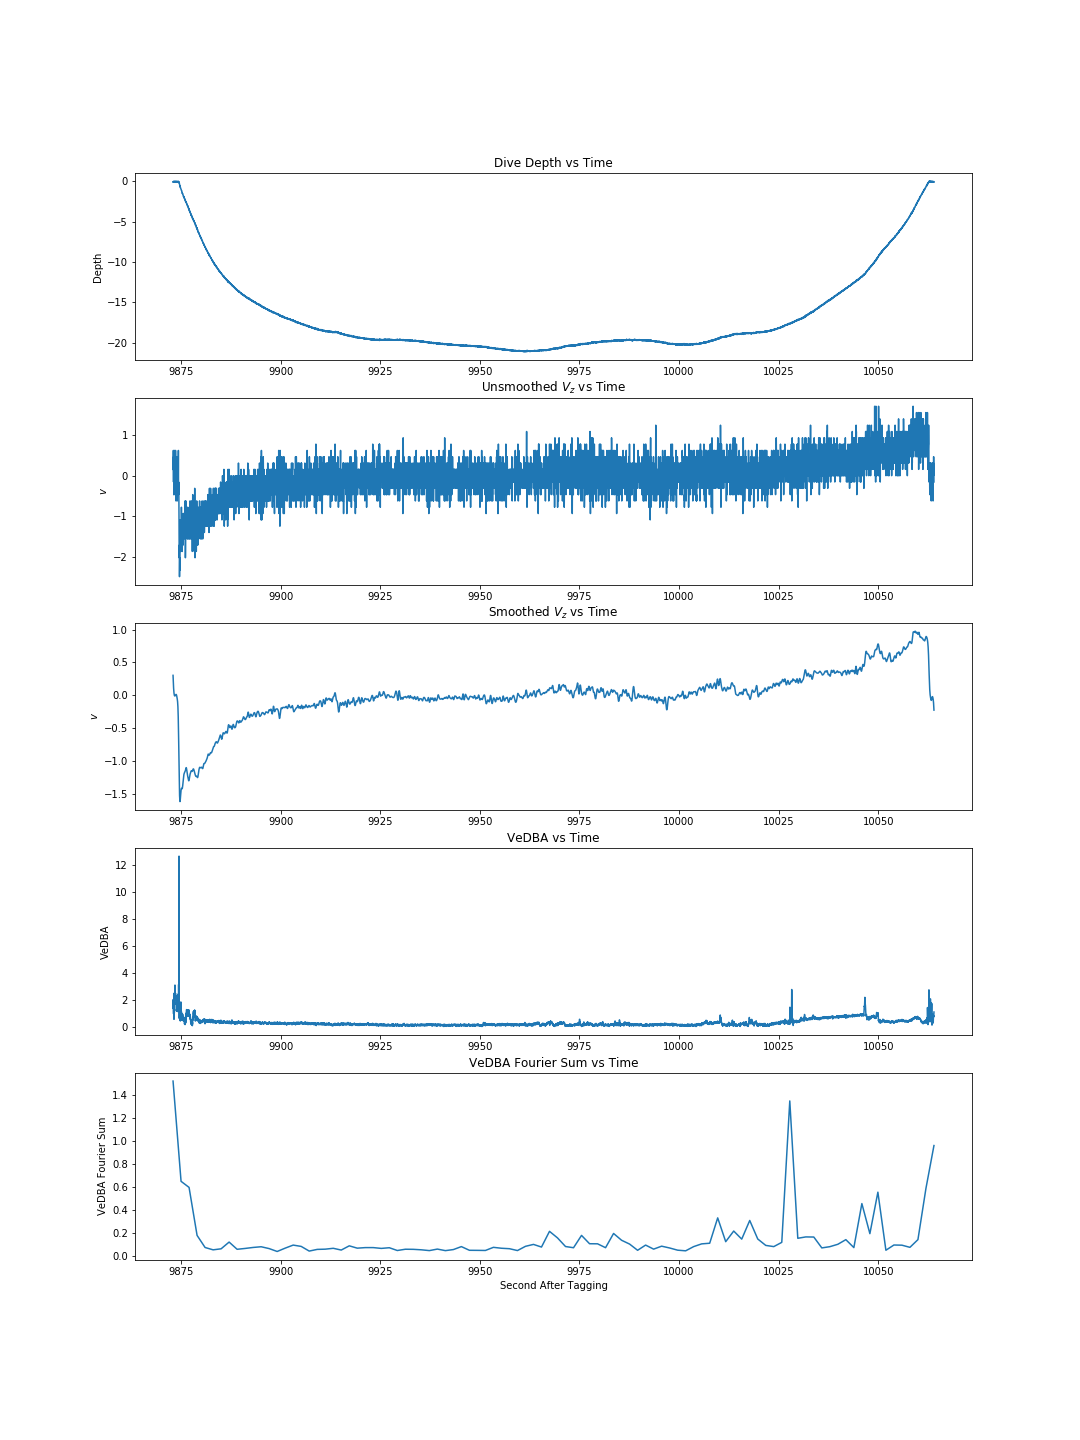
\includegraphics[height=7.5in]{../Plots/smoothed_v.png}
	\caption{From top to bottom: dive depth, unsmoothed vertical velocity, smoothed vertical velocity, ODBA, and the sum of low-frequency Fourier coefficeints of the ODBA for a randomly selected dive of a killer whale.}
	\label{fig:smoothing}
\end{figure}

Figure (\ref{fig:smoothing}) also shows the calculated ODBA as a function of time for one a specific dive. The acceleration exhibits sinusoidal behavior at several points in time which cannot be modeled using HMMs straightforwardly. As a result, the data was split into two-second intervals (100 data points each), and each interval was summarized by the Fourier transform of the ODBA and the velocity at the \textit{end} of the time interval. Velocity was taken at the end of the time interval because the behavior of the whale during the time interval has no impact on the velocity of the whale at the beginning of the time interval. Because velocity is highly correlated with the average acceleration within an interval, the mean was subtracted out of each ODBA time series before the Fourier transform was taken. To reduce the dimension of the ODBA Fourier transform, Fourier coefficients corresponding to frequencies less than or equal to 5 hertz were summed and frequencies above 5 hertz were ignored. One nice property of this process is that it reduces the number of data points by a factor of 100, which drastically speeds up parameter estimation. The optimal length of the time interval over which to take the Fourier transform is a tuning parameter that is difficult to find. An ideal time interval should be long enough give useful Fourier coefficients, but short enough to preserve as much information about the vertical velocity of the animal as possible.

\subsection{Lag Plot}

In order to find the appropriate HMM to model whale behavior, a lag plot was made for both velocity and the ODBA fourier sum. The results of doing so are shown in figure (\ref{fig:lag}). Unfortunately, the number of behavioral states is not clear from the lag plot, but it is clear that the velocity exhibits a large degree of autocorrelation. While the ODBA Fourier sum also exhibits some autocorrelation, the relationship is less strong, so autocorrelation was not incorporated in the ODBA Fourier sums emission distribution.